%
% File acl2013.tex
%
% Contact  navigli@di.uniroma1.it
%%
%% Based on the style files for ACL-2012, which were, in turn,
%% based on the style files for ACL-2011, which were, in turn, 
%% based on the style files for ACL-2010, which were, in turn, 
%% based on the style files for ACL-IJCNLP-2009, which were, in turn,
%% based on the style files for EACL-2009 and IJCNLP-2008...

%% Based on the style files for EACL 2006 by 
%%e.agirre@ehu.es or Sergi.Balari@uab.es
%% and that of ACL 08 by Joakim Nivre and Noah Smith

\documentclass[11pt]{article}
\usepackage{style}
\usepackage{times}
\usepackage{latexsym}
\usepackage[utf8]{inputenc}
\usepackage{listings}
\usepackage{multicol}
\usepackage{graphicx}
\usepackage{lmodern}
\usepackage{color}
\usepackage{url}
%\setlength\titlebox{6.5cm}    % You can expand the title box if you
% really have to

\definecolor{darkgreen}{rgb}{0,0.7,0}
\definecolor{lightgray}{gray}{0.6}

\lstset{
	language=Java,                 % the language of the code
	basicstyle=\fontsize{8}{8}\ttfamily,        % the size of the fonts that are used for the code
	showstringspaces=false,
	commentstyle=\color{darkgreen},    % comment style
	extendedchars=true,              % lets you use non-ASCII characters; for 8-bits encodings only, does not work with UTF-8
	keepspaces=true,                 % keeps spaces in text, useful for keeping indentation of code (possibly needs columns=flexible)
	breaklines=true,  
	morekeywords={function, var, using, include, namespace},
	keywordstyle=\color{blue},       % keyword style
	numbers=none,                    % where to put the line-numbers; possible values are (none, left, right)
	numbersep=5pt,                   % how far the line-numbers are from the code
	numberstyle=\color{lightgray}, % the style that is used for the line-numbers
	stepnumber=1,                    % the step between two line-numbers. If it's 1, each line will be numbered
	showspaces=false, 
	stringstyle=\color{red},     % string literal style
	tabsize=2,	                   % sets default tabsize to 2 spaces
	captionpos=b,
	 frame=ltbr,
}

\title{Modern Tools in Machine Learning.}

\author{Samuel Schepp \\
  Technische Hochschule Mittelhessen \\
  Fachbereich MNI \\
  Master-Seminar \\
  {\tt samuel.schepp@mni.thm.de} \\
  }

\date{}

\begin{document}
\maketitle
\begin{abstract}
This paper introduces common machine learning tools like TensorFlow, PyCharm, and PyPlot, which are used to setup and run machine learning tasks with neural networks.
A common "Hello World" script will be developed to show the concept and ideas of these tools.
It will make use of the "Fashion MNIST dataset" by Zalando, which will be explored in detail.

In addition, there will be shown, how to run trainings on a graphics card and what TensorFlow is not doing.

\end{abstract}

\section{MNIST Datasets}

To get started with machine learning, there needs to be data that a model can read and produces a result of.
In addition, a model needs much more data to train.
In the "Hello World" example, which will be developed later, there will be used the "Fashion MNIST dataset", which is created by Zalando, an online fashion store.
Zalando is developing solution, which can detect and classify pictures of cloth.
Their current focus is machine learning.

A MNIST dataset contains four individual sets.
The first set is a list of images, which will be used to train on.
The second set is a list of class names, that refers to the actual thing, that is shown on the image at the same index.
That means, that image 4 might show a jacket, the class name on set 2, index 4 says "jacket".
These two datasets can now be used to train a model, which should recognize the image.

The remaining two datasets are again pictures and class names of cloth.
These are used to test the model.
The images are new and different ones, to make sure, the model is not over fitting.
Over fitting means, that the model is only capable of recognizing the given dataset, but is likely to fail on unknown and new pictures.

\subsection{Origin}

The acronym "MNIST" database stands for "Modified National Institute of Standards and Technology database".
It is a large database of handwritten digits, that is used to train neural networks and image processing systems.
There are 60,000 training and 10,000 testing images, which are normalized, centered and 28 by 28 pixel in size.
It is easy for convolutional neural networks, to classify these images at a failure rate of under 1 percent.

The images are encoded in a simple byte-array based format, so no conventional image application can open them.
TensorFlow is able to decode the images and use them as input, since it became a common format.


\begin{figure}[h]
\caption{The original MNIST database with handwritten digits}
\centering
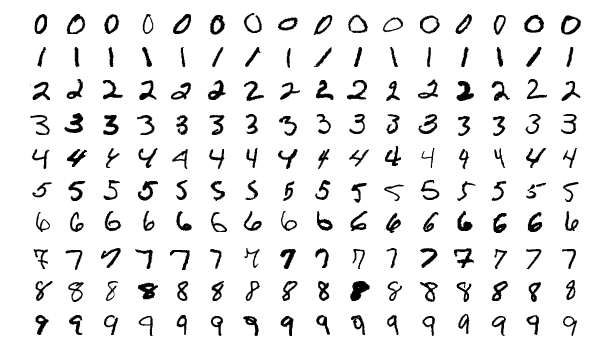
\includegraphics[width=0.5\textwidth]{img/mnist_example.png}
\end{figure}

\subsection{Examples}

Since the MNIST database is popular amongst machine learning scientists, it became a standard format for other content.
Zalando uses it, to provide example data to the public and try out different learning systems.

They created a database which contains clothing and its names (class).
It has a size of 26 MB for training and 4.3 MB for test samples.
There are 10 classes of clothing:  T-shirt/top, trouser, pullover, dress, coat, sandal, shirt, sneaker, bag and ankle boot.
It is not a coincidence, that the count of classes here is the same as the original set, which contains handwritten digits.
A system, that can train the handwriting, can also train and recognize the clothing, without any reimplementation.

\begin{figure}[h]
\caption{Snippet of the Zalando fashion MNIST.}
\centering
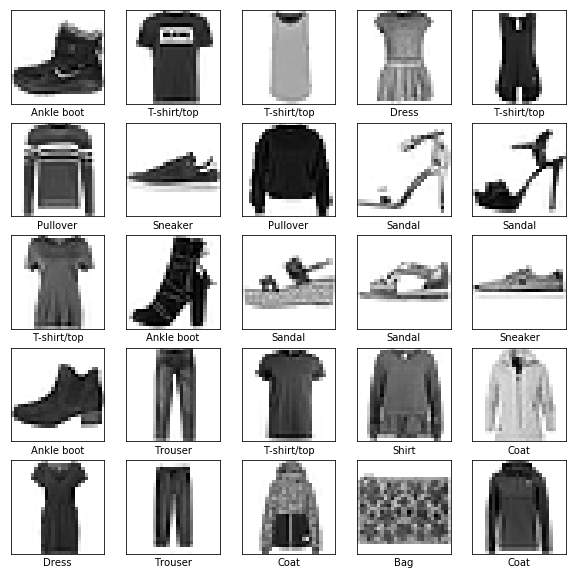
\includegraphics[width=0.5\textwidth]{img/mnist_fashion.png}
\end{figure}

TensorFlow is able to directly load the fashion MNIST, since it is part of the python package.

\begin{lstlisting}[caption={Loading the fashion MNIST in TensorFlow (Python)}, language=Python]
from tensorflow import keras

fashion_mnist = keras.datasets.fashion_mnist
(train_images, train_labels), (test_images, test_labels) = fashion_mnist.load_data()
\end{lstlisting}

The tuples contain TensorFlow-friendly data, that can directly be used in Keras, which is TensorFlow's high level API to configure and run neural networks.

\section{TensorFlow}

TensorFlow is a software platform for numerical computation, with focus on neural networks and deep learning.
It is developed by Google's AI organization and provides frameworks for many scientific domains.

It provides hardware accelaration for graphics cards and it own chips called "TensorFlow Processing Unit" (TPU).

Most of the time, the Python package is adequate to perform many basic and advanced machine learning tasks.

\subsection{Keras}

The Pyhton package of TensorFlow contains Keras, which is a high level interface to several deep learning back ends, like Theano, Microsoft Cognitive Toolkit and TensorFlow.

It is the default API for TensorFlow, although it is a independent open source project.
That means you will be able to run deep learning algorithms, that are developed for TensorFlow, on different frameworks.

\subsection{TensorFlow.js}

\subsection{TensorFlow lite}

\subsection{Limits}

\section{PyPlot}

\section{Hardware Acceleration}

\section{Hello World}


\begin{thebibliography}{1}

\bibitem{node}Fashion-MNIST

\url{https://github.com/zalandoresearch/fashion-mnist}

Accessed: 2019-01-12.

\bibitem{node}Zalando Research

\url{https://research.zalando.com}

Accessed: 2019-01-12.


\bibitem{node}MNIST Database

\url{http://yann.lecun.com/exdb/mnist/}

Accessed: 2019-01-12.


\bibitem{node}TensorFlow Processing Unit

\url{https://cloud.google.com/tpu/?hl=de}

Accessed: 2019-01-12.

\end{thebibliography}

\end{document}

